\documentclass[10pt]{article}

\usepackage[margin=0.78in]{geometry}
\usepackage{fontspec}
\usepackage{amsmath,amssymb,amsthm,mathtools}
\usepackage{booktabs,array}
\usepackage{enumitem}
\usepackage{graphicx}
\usepackage{xcolor}
\usepackage{microtype}
\usepackage[colorlinks=true,linkcolor=blue!55!black,citecolor=blue!55!black,urlcolor=blue!55!black]{hyperref}

\graphicspath{{./}{./toricgt_pg_softmoe_figures/}}

\theoremstyle{definition}
\newtheorem{definition}{Definition}
\newtheorem{assumption}[definition]{Assumption}
\theoremstyle{plain}
\newtheorem{theorem}[definition]{Theorem}
\newtheorem{lemma}[definition]{Lemma}
\newtheorem{proposition}[definition]{Proposition}
\newtheorem{corollary}[definition]{Corollary}
\theoremstyle{remark}
\newtheorem{remark}[definition]{Remark}

\newcommand{\R}{\mathbb R}
\newcommand{\Z}{\mathbb Z}
\newcommand{\Q}{\mathbb Q}
\newcommand{\A}{\mathcal A}
\newcommand{\G}{\mathcal G}
\newcommand{\Eop}{\mathbb E}
\newcommand{\softmax}{\operatorname{softmax}}
\newcommand{\argmax}{\operatorname*{arg\,max}}
\newcommand{\Conv}{\operatorname{Conv}}
\newcommand{\Newt}{\operatorname{Newt}}
\newcommand{\norm}[1]{\left\lVert #1\right\rVert}
\newcommand{\ip}[2]{\left\langle #1,#2\right\rangle}
\newcommand{\transpose}{^{\mathsf T}}

\title{\vspace{-1.4em}ToricGT: Compact Graph-Token Reasoning with Tropical Ring Attention, Toric Diagnostics, and Random-Order Compression}
\author{Amelie Schreiber}
\date{}

\begin{document}
\maketitle

\begin{abstract}
We present ToricGT, a compact graph-to-graph Transformer family for algebraic, mathematical, morphological, and parameter-constrained language-model reasoning.  The research model tokenizes nodes and edges as a shared sequence, uses exact blockwise ring evaluation for tropical max-plus attention, adds finite noncommutative-torus phase channels, and uses permutation-equivariant Soft-MoE routing in upper graph blocks.  The paper contributes a finite theory and an implementation-facing training contract.  We prove graph-token equivariance, exactness of tropical ring attention, stability of active faces under perturbation, and simulation of bounded semiring dynamic programs.  Motivated by recent toric geometry of ReLU networks, we further interpret tropical head decisions as active faces of Newton polytopes and normal fans, giving compact diagnostics for margins, bends, and future toric auxiliary losses.  A separate OpenAI Parameter-Golf track projects byte chunks to random-order graph positions and trains a dense recurrent micro language model with tied embeddings, toric position phases, tropical-ring attention, compact noncommutative-toric memory, strict-prefix GFlowNet graph-of-thought actions, BigramHash/CaseOps byte features, SmearGate confidence, stripped multi-token auxiliary heads, score-first test-time bias adaptation, and bit-packed 6-bit row-quantized export.  The result is a small, auditable model design whose reasoning behavior is inspected through equivariance errors, active faces, toric moments, artifact bytes, BPB, and GFlowNet diversity rather than scalar accuracy alone.
\end{abstract}

\section{Introduction}

Many reasoning tasks are naturally graph-to-graph transformations: proof steps depend on earlier equations, graph algorithms update node and edge states, Hebrew morphology links surface forms to roots and templates, and algebraic words reduce through local rewrite relations.  ToricGT targets this regime with three design constraints.  First, relabeling a graph should relabel node and edge outputs, not change the computation.  Second, dynamic-programming-like reasoning should be visible through max-plus active faces and margins.  Third, compactness matters: the same ideas should support a small research model and a Parameter-Golf-style byte model under a strict artifact budget.

\begin{figure}[t]
  \centering
  
\includegraphics[width=\linewidth]{toricgt_architecture_and_training_diagram.png}
  \caption{ToricGT combines graph tokenization, tropical ring attention, noncommutative-torus phase channels, Soft-MoE routing, and embedding-space GFlowNet fine-tuning.}
  \label{fig:arch-condensed}
\end{figure}

The main novelty is the integration of algebraic structure with trainable graph-token Transformers.  Tropical attention implements max-plus gates and exposes provenance.  Ring evaluation changes the schedule but not the function.  Finite Weyl pairs encode projective toric phase memory.  Soft-MoE gives typed differentiable routing in the research graph model.  For Parameter Golf, the same graph-token idea is compressed into random-order autoregressive decoding: each byte position becomes a graph node scored in a content-independent random order.  Finally, toric geometry supplies a new diagnostic layer: active candidates in tropical heads form exposed faces of Newton polytopes, and changes across cell walls behave like bend or Cartier-divisor intersection measurements.

\section{Model}

A ToricGT instance is
\begin{equation}
  F(G)=D\circ \Phi_L\circ\cdots\circ\Phi_1\circ T(G),
\end{equation}
where $T$ maps a typed attributed graph to node and edge tokens, $\Phi_\ell$ is a shared token-equivariant block, and $D$ is a shared node/edge/graph decoder.  A graph is
\begin{equation}
  G=(V,E,s,t,\tau_V,\tau_E,x,e,m_V,m_E),
\end{equation}
with source and target maps for edge tokens, finite node and edge types, bounded attributes, and padding masks.

\paragraph{Tropical ring attention.}
For score matrix $S$ and values $V$, a tropical head computes
\begin{equation}
  Y_{ic}=\max_j(S_{ij}+V_{jc}),\qquad
  A_{ic}=\argmax_j(S_{ij}+V_{jc}).
\end{equation}
Partitioning keys into blocks $B_1,\ldots,B_R$ gives
\begin{equation}
  \max_j(S_{ij}+V_{jc})
  =
  \max_r\max_{j\in B_r}(S_{ij}+V_{jc}),
\end{equation}
so ring evaluation is exactly equal to full tropical attention in exact arithmetic.

\paragraph{Soft-MoE routing.}
For hidden states $X\in\R^{B\times L\times d}$, learned slot vectors $\Phi\in\R^{d\times E\times S}$, and validity mask $M$, define
\begin{align}
  A_{bies}&=g\ip{x_{bi}/\norm{x_{bi}}}{\phi_{es}/\norm{\phi_{es}}},\\
  D_{bies}&=\frac{\exp A_{bies}M_{bi}}{\sum_j\exp A_{bjes}M_{bj}+\epsilon},\\
  C_{bies}&=\frac{\exp A_{bies}}{\sum_{e',s'}\exp A_{bie's'}+\epsilon},\\
  Z_{bes}&=\sum_iD_{bies}X_{bi},\qquad
  Y_{bi}=\sum_{e,s}C_{bies}f_e(Z_{bes}).
\end{align}
We use $E\ge4$ experts by default in the graph model.  The Parameter-Golf micro-LM is dense by default because a full expert bank is usually a poor bytes-per-quality tradeoff under a 16 MB artifact cap; prefix-causal or low-rank Soft-MoE remains an ablation after the dense baseline is stable.

\section{Theory}

\begin{theorem}[Graph equivariance]
If tokenization, masks, attention projections, tropical heads, Soft-MoE routing, residuals, normalization, and decoders are shared over token rows and use only equivariant incidence/type information, then ToricGT is graph-to-graph equivariant.
\end{theorem}

\begin{proof}
Tokenization maps relabeled graphs to row-permuted token tables.  Linear projections commute with row permutations.  Softmax attention, tropical attention, and Soft-MoE dispatch/combination commute with the same row permutation because their normalizers sum over either all valid tokens or slots for a fixed token.  Row-wise residual, normalization, and decoder maps commute with permutations.  Composition preserves equivariance.
\end{proof}

\begin{lemma}[Active-face stability]
If $\norm{S-\widehat S}_\infty\le\epsilon_S$ and $\norm{V-\widehat V}_\infty\le\epsilon_V$, then tropical outputs obey
\begin{equation}
  \norm{Y-\widehat Y}_\infty\le\epsilon_S+\epsilon_V.
\end{equation}
If the top-two margin is larger than $2(\epsilon_S+\epsilon_V)$, the active key is unchanged.
\end{lemma}

\begin{proof}
Each candidate score changes by at most $\epsilon_S+\epsilon_V$, and the maximum is 1-Lipschitz in $\ell_\infty$.  The margin condition keeps the original maximizer strictly above all competitors after perturbation.
\end{proof}

\paragraph{Toric diagnostic theorem.}
Let a tropical probe be $\psi(h)=\max_r(\ip{a_r}{h}+b_r)$ with rational slopes $a_r$.  Its Newton polytope is $P=\Conv(a_1,\ldots,a_R)$.  The active set
\begin{equation}
  A(h)=\argmax_r(\ip{a_r}{h}+b_r)
\end{equation}
is the exposed face of the lifted polytope $\Conv\{(a_r,b_r)\}_r$ under the linear functional $(a,b)\mapsto\ip{a}{h}+b$.  Hence tropical active-face diagnostics are cells of a normal fan.  This imports the ReLU fan / Cartier-divisor viewpoint of Fu \cite{fu2025toricrelu} into ToricGT tropical subcomputations, complementing earlier tropical rational interpretations of ReLU networks \cite{zhang2018tropical}.

\begin{figure}[t]
  \centering
  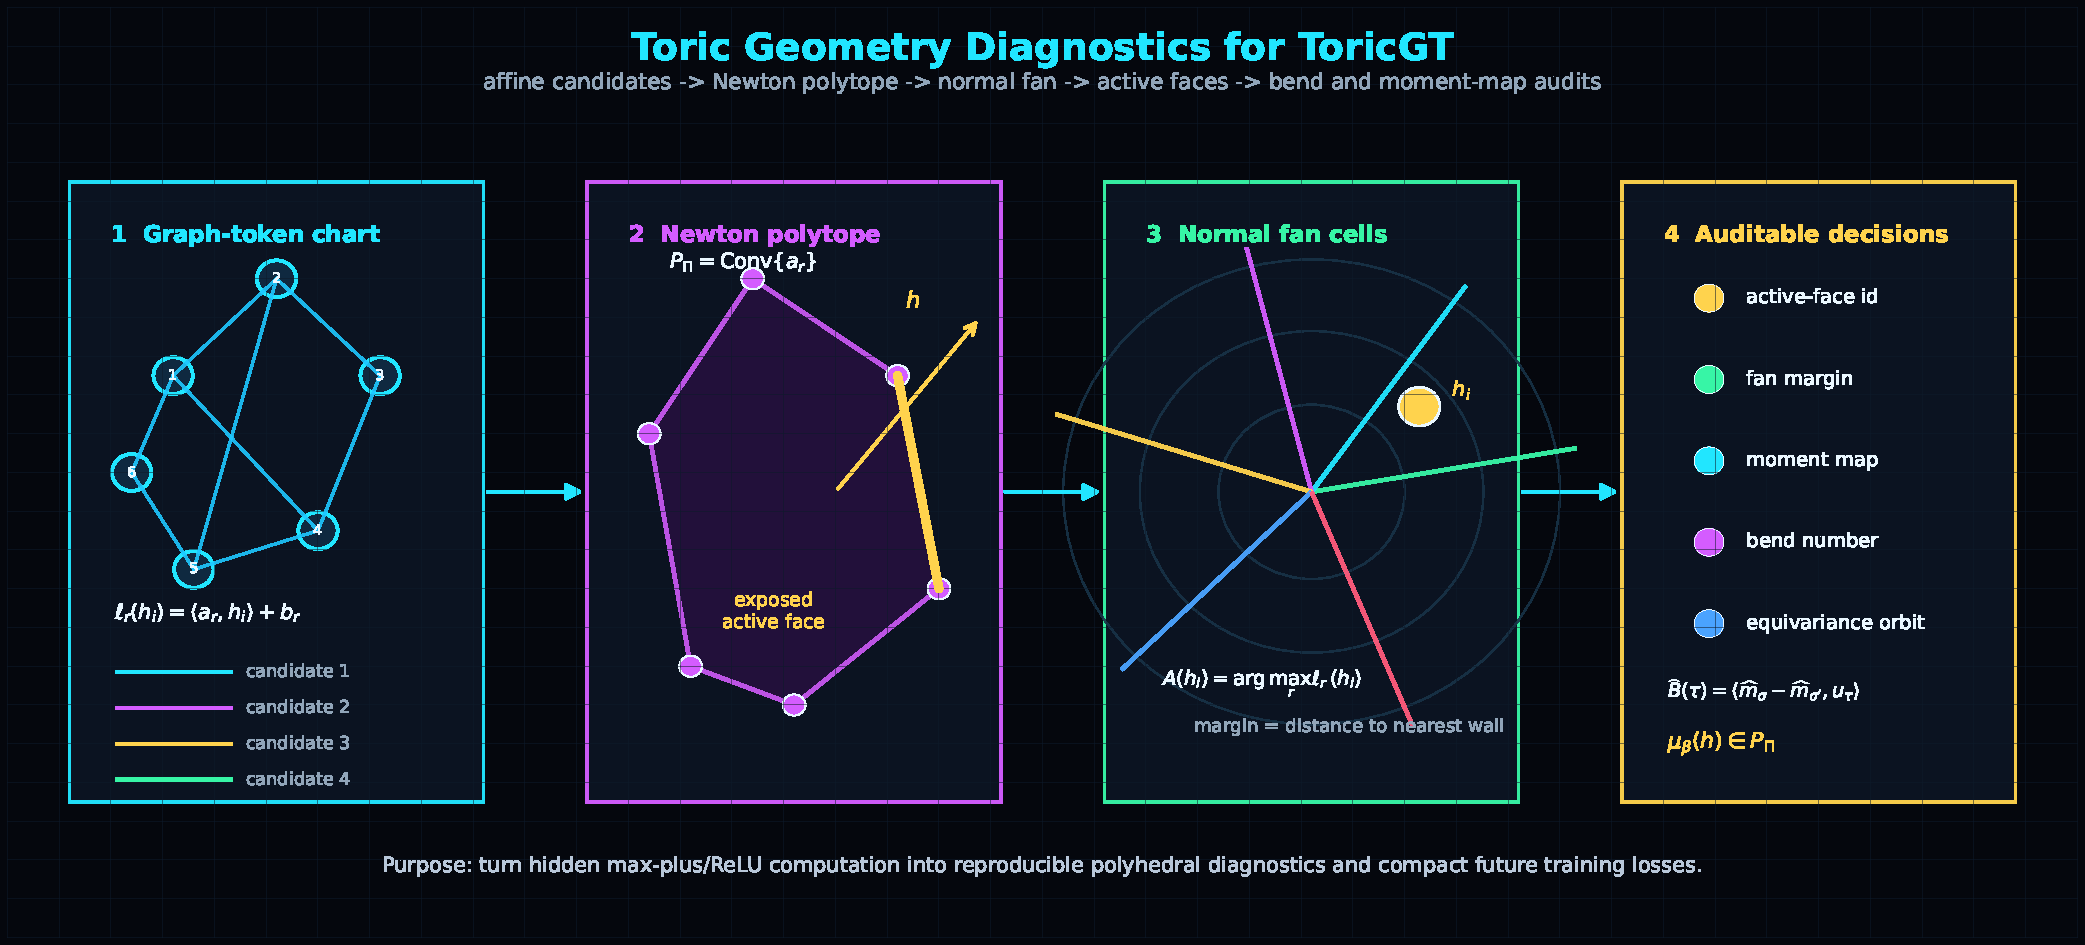
\includegraphics[width=\linewidth]{fig_toric_geometry_relu_toricgt.pdf}
  \caption{Toric diagnostics turn tropical candidate scores into Newton polytopes, normal-fan cells, active-face margins, and bend measurements.}
  \label{fig:toric-condensed}
\end{figure}

\paragraph{Finite noncommutative-toric memory.}
Let $\theta,\beta$ be rationally independent.  The competition adapter stores a small memory bank indexed by
\begin{equation}
  m_s=(\sin 2\pi s\theta,\cos 2\pi s\theta,\sin 2\pi s\beta,\cos 2\pi s\beta,
  \sin(2\pi s\theta+2\pi s\beta+2\pi s^2\theta),\cos(2\pi s(\theta-\beta))).
\end{equation}
The quadratic phase term is a finite cocycle surrogate: it gives a compact, byte-accounted way to expose clock/shift-like projective phase structure without claiming a faithful finite representation of an irrational rotation algebra.  Queries attend to these slots by cosine attention and add a small residual before logits.

\begin{proposition}[Ergodic phase coverage]
If $1,\theta,\beta$ are rationally independent, the sequence $(s\theta,s\beta)\bmod1$ is equidistributed on $\mathbb T^2$.  Consequently, finite prefixes of the toric memory supply low-discrepancy phase probes as the number of slots grows.
\end{proposition}

\begin{proof}
This is Kronecker-Weyl equidistribution.  For any nonzero $k\in\mathbb Z^2$, rational independence gives $k_1\theta+k_2\beta\notin\mathbb Z$, so the exponential averages $n^{-1}\sum_{s<n}\exp(2\pi i s(k_1\theta+k_2\beta))$ vanish.  Weyl's criterion implies equidistribution.
\end{proof}

\paragraph{Hidden-flow regularization.}
Embedding reasoning paths are treated as discrete flows $h_0,\ldots,h_T$.
Let $u_t=h_t-h_{t-1}$ and $\Delta u_t=u_t-u_{t-1}$.  The competition branch adds
\begin{align}
  \mathcal L_{\mathrm{flow}}
  &=
  \Eop_t\|\Delta u_t\|_2^2
  +\nu \Eop_t\|u_t\|_2^2 \nonumber\\
  &\quad
  +10^{-3}\operatorname{Var}_t\|h_t\|_2.
\end{align}
This is not a fluid simulation.  It is a Navier--Stokes-inspired discrete dissipation prior: high-frequency trajectory oscillations are penalized, but smooth transport through embedding space remains cheap.  The regularizer improves the stability of long GFlowNet reasoning paths and provides kinetic-energy and viscous-dissipation diagnostics for the 3D trajectory and energy-landscape plots.

\section{Training And Evaluation}

The supervised objective combines node, edge, and graph losses with equivariance, torus, tropical-margin, Hebrew morphology, Soft-MoE, cache, and distillation terms:
\begin{equation}
\begin{split}
\mathcal L={}&\lambda_V\mathcal L_V+\lambda_E\mathcal L_E+\lambda_G\mathcal L_G
+\lambda_{\mathrm{eq}}\mathcal L_{\mathrm{eq}}
+\lambda_\Theta\mathcal L_\Theta+\lambda_{\mathrm{trop}}\mathcal L_{\mathrm{margin}}\\
&+\lambda_H\mathcal L_H+\lambda_{\mathrm{moe}}\mathcal L_{\mathrm{moe}}
+\lambda_{\mathrm{cache}}\mathcal L_{\mathrm{PQ}}
+\lambda_{\mathrm{KD}}\mathcal L_{\mathrm{distill}}.
\end{split}
\end{equation}
Embedding-space GFlowNet fine-tuning samples reasoning graphs with probability proportional to reward using trajectory balance.  The reward combines correctness, novelty, low equivariance error, tropical margin, low toric commutator error, and complexity penalties.

The data mixture is graph-first: math reasoning, graph-of-thought traces, algorithmic tasks, synthetic rotation/tropical tasks, Hebrew morphology graphs, and Jewish Hebrew text sources are normalized into Parquet records with stable content hashes and graph JSON.  Splits are clustered by near-duplicate text, graph sketches, algebraic normal forms, root families, and source references.

\begin{center}
\begin{tabular}{p{0.31\linewidth}p{0.53\linewidth}}
\toprule
Metric & Failure mode exposed \\
\midrule
Equivariance error & absolute-position leakage and edge-order bugs \\
Active-face margin & unstable dynamic-programming decisions \\
Toric bend consistency & incoherent polyhedral reasoning changes \\
Soft-MoE expert mass & expert collapse or over-routing \\
GFlowNet diversity & mode collapse and reward hacking \\
Parameter-Golf BPB/bytes & compactness and scoring compliance \\
\bottomrule
\end{tabular}
\end{center}

\section{Parameter-Golf Track}

The contest-facing model is not the full graph encoder.  It is a dense random-order byte model with tied embeddings, recurrent block reuse, toric target-position phases, lower softmax attention, upper tropical-ring attention, compact prefix-visible GFlowNet action sampling, noncommutative-toric memory slots, and byte-accounted export.  The artifact budget is
\begin{equation}
  B_{\mathrm{art}}=B_{\mathrm{code}}+B_{\mathrm{weights}}+B_{\mathrm{tokenizer}}+B_{\mathrm{metadata}}
  \le16{,}000{,}000.
\end{equation}
For a byte chunk $b=(b_1,\ldots,b_T)$, sample a content-independent order $\pi\in S_T$ from public metadata and factor
\begin{equation}
  q_\theta(b\mid \pi)=\prod_{k=1}^Tq_\theta(b_{\pi_k}\mid b_{\pi_{<k}},\pi_{\le k}).
\end{equation}
BPB is computed prequentially: predict a normalized next-byte distribution, score the observed byte, then update the state.  Because $\pi$ is independent of unscored byte values and row $k$ never contains $b_{\pi_k}$, random-order decoding is score-before-update valid while exposing more graph-like order diversity than ordinary left-to-right decoding.  A byte-safe GFlowNet policy samples latent graph-of-thought action embeddings from the prefix-visible hidden state, and validation can average multiple action samples.  Dense recurrence is the default because it adds computation without adding stored expert weights; Soft-MoE adapters are retained only as byte-accounted ablations.  Curated \texttt{graph\_json} records are projected into compact node/edge byte traces so graph structure is visible to this adapter.

The current competition branch adds several high-impact modifications inspired by OpenAI's public Parameter-Golf retrospective while excluding JEPA.  BigramHash gives a tiny strict-prefix n-gram memory; CaseOps adds byte-class operator features; SmearGate learns input-dependent confidence; stripped multi-token heads improve hidden states but are omitted from the artifact; contrastive hidden-state regularization replaces JEPA-style prediction; coprime row striding changes data order without changing data; score-first output-bias adaptation updates only after a token has been scored; and bit-packed 6-bit row quantization with LZMA reduces serialized weight cost.  Domain tags emphasize math, code, graph, Hebrew, biomedical, biochemical, biophysical, and toric records without adding evaluator dependencies.

Operationally, the first serious BPB target is $1.20$--$1.22$, a strong run is $1.16$--$1.19$, an excellent run is $1.13$--$1.15$, and $\le1.12$ is exceptional under OpenAI's public recap.  Claims below $1.10$ BPB should trigger strict leakage, tokenizer, and score-before-update audits.

\section{Next Iteration}

The next ToricGT iteration should use toric geometry as a training signal.  First, freeze the trained checkpoint and build empirical toric shadows: occupied fan cells, fitted slopes, active-face margins, and bend magnitudes.  Second, add synthetic toric tasks: Newton-polytope active-face prediction, Cartier-divisor bend prediction, toric ideal relation checks, and ReLU fan realization tests.  Third, attach low-rank quantized toric probes and optimize
\begin{equation}
  \mathcal L_{\mathrm{toric}}
  =
  \mathcal L_{\mathrm{base}}
  +\lambda_{\mathrm{fan}}\mathcal L_{\mathrm{fan}}
  +\lambda_{\mathrm{bend}}\mathcal L_{\mathrm{bend}}
  +\lambda_{\mathrm{binom}}\mathcal L_{\mathrm{binom}}
  +\lambda_{\mathrm{moment}}\norm{\widehat\mu-\mu^\star}_2^2.
\end{equation}
Finally, make inference-time scaling geometric: continuous GFlowNets can move inside normal cones, along walls, and across moment polytopes while discrete actions edit graph-of-thought states.  Continuous GFlowNet theory supplies the density-correct trajectory-balance objective for these hybrid paths \cite{lahlou2023continuous}.  This keeps the architecture small while giving search a structured latent space.

\section{Conclusion}

ToricGT is a finite, auditable model family.  Its exact claims are graph-token equivariance, ring-schedule exactness, max-plus semiring simulation on bounded domains, projective toric phase consistency, random-order score validity for byte modeling, and perturbation bounds for compressed caches.  Its practical claim is that reasoning models should expose the geometry of their decisions.  Tropical active faces, Newton polytopes, toric bends, artifact bytes, BPB, expert utilization, and GFlowNet reward landscapes make small-model reasoning easier to test, compress, and improve.

\begin{thebibliography}{99}

\bibitem{fu2025toricrelu}
Yaoying Fu.
\newblock Toric geometry of ReLU neural networks.
\newblock arXiv:2509.05894, 2025.

\bibitem{zhang2018tropical}
Liwen Zhang, Gregory Naitzat, and Lek-Heng Lim.
\newblock Tropical geometry of deep neural networks.
\newblock In \emph{ICML}, PMLR 80:5824--5832, 2018.

\bibitem{kim2022tokengt}
Jinwoo Kim, Tien Dat Nguyen, Seonwoo Min, Sungjun Cho, Moontae Lee, Honglak Lee, and Seunghoon Hong.
\newblock Pure Transformers are powerful graph learners.
\newblock \emph{NeurIPS}, 2022.

\bibitem{liu2023ring}
Hao Liu, Matei Zaharia, and Pieter Abbeel.
\newblock Ring Attention with blockwise Transformers for near-infinite context.
\newblock arXiv:2310.01889, 2023.

\bibitem{puigcerver2024softmoe}
Joan Puigcerver, Carlos Riquelme, Basil Mustafa, and Neil Houlsby.
\newblock From Sparse to Soft Mixtures of Experts.
\newblock \emph{ICLR}, 2024.

\bibitem{bengio2023gflownet}
Yoshua Bengio, Salem Lahlou, Tristan Deleu, Edward J. Hu, Mo Tiwari, and Emmanuel Bengio.
\newblock GFlowNet foundations.
\newblock \emph{JMLR}, 24(210):1--55, 2023.

\bibitem{lahlou2023continuous}
Salem Lahlou, Tristan Deleu, Pablo Lemos, Dinghuai Zhang, Alexandra Volokhova, Alex Hern\'andez-Garc\'ia, Lena Nehale Ezzine, Yoshua Bengio, and Nikolay Malkin.
\newblock A theory of continuous generative flow networks.
\newblock In \emph{ICML}, PMLR 202:18269--18300, 2023.

\bibitem{han2025polarquant}
Insu Han, Praneeth Kacham, Amin Karbasi, Vahab Mirrokni, and Amir Zandieh.
\newblock PolarQuant: Quantizing KV Caches with Polar Transformation.
\newblock arXiv:2502.02617, 2025.

\bibitem{brandenburg2024real}
Marie-Charlotte Brandenburg, Georg Loho, and Guido Montufar.
\newblock The real tropical geometry of neural networks.
\newblock arXiv:2403.11871, 2024.

\end{thebibliography}

\end{document}
